%%%%%%%%%%%%%%%%%%%%%%%%%%%%%%%%%%%%%%%%%
% University/School Laboratory Report
% LaTeX Template
% Version 3.0 (4/2/13)
%
% This template has been downloaded from:
% http://www.LaTeXTemplates.com
%
% Original author:
% Linux and Unix Users Group at Virginia Tech Wiki 
% (https://vtluug.org/wiki/Example_LaTeX_chem_lab_report)
%
% License:
% CC BY-NC-SA 3.0 (http://creativecommons.org/licenses/by-nc-sa/3.0/)
%
%%%%%%%%%%%%%%%%%%%%%%%%%%%%%%%%%%%%%%%%%

%----------------------------------------------------------------------------------------
%	PACKAGES AND DOCUMENT CONFIGURATIONS
%----------------------------------------------------------------------------------------

\documentclass{article}

%\usepackage{mhchem} % Package for chemical equation typesetting
%\usepackage{siunitx} % Provides the \SI{}{} command for typesetting SI units

\usepackage{graphicx} % Required for the inclusion of images
\usepackage[top=1in,bottom=1in,right=1in,left=1in]{geometry}% Set the margins

%Multiple column picture packages
\usepackage{caption}
\usepackage{subcaption}

%Add code formating
%\usepackage{listings}
%\lstset{tabsize=2}

%Add support for floating images
\usepackage{float}

%Define the style for VHDL
%\lstdefinelanguage{VHDL}{
%  morekeywords={
%    library,use,all,entity,is,port,in,out,end,architecture,of,
%    begin,and
%  },
%  morecomment=[l]--
%}

%Give the VHDL code color
%\usepackage{xcolor}
%\colorlet{keyword}{blue!100!black!80}
%\colorlet{comment}{green!90!black!90}
%\lstdefinestyle{vhdl}{
%  language     = VHDL,
%  basicstyle   = \ttfamily,
%  keywordstyle = \color{keyword}\bfseries,
%  commentstyle = \color{comment}
%}

\usepackage{amssymb}
\usepackage{amsmath}

%Highlight command
%\usepackage{tikz}
%\usepackage{xspace}
%\usetikzlibrary{decorations.pathmorphing}
%\newcommand\hl[1]{%
%    \tikz[baseline,%
%      decoration={random steps,amplitude=1pt,segment length=15pt},%
%      outer sep=-15pt, inner sep = 0pt%
%    ]%
%   \node[decorate,rectangle,fill=yellow,anchor=text]{#1\xspace};%
%}%

% Create the header and footer
\usepackage{fancyhdr}
\pagestyle{fancy}
\lhead{CprE 583}
\rhead{Blake Vermeer, Kris Hall, Rohit Zambre}
\renewcommand{\footrulewidth}{0.4pt}

\setlength\parindent{0pt} % Removes all indentation from paragraphs

\renewcommand{\labelenumi}{\alph{enumi}.} % Make numbering in the enumerate environment by letter rather than number (e.g. section 6)

%\usepackage{times} % Uncomment to use the Times New Roman font

%----------------------------------------------------------------------------------------
%	DOCUMENT INFORMATION
%----------------------------------------------------------------------------------------

\title{MP-3 Write-Up} % Add title here...

\author{Blake \textsc{Vermeer}\\
		Kris \textsc{Hall}\\
		Rohit \textsc{Zambre}} % Author name

\date{\today} % Date for the report

\begin{document}

\maketitle % Insert the title, author and date

\begin{center}
\begin{tabular}{l r}
Date Due: & October 31, 2014 \\ % Date the assignment is due
%Partners: & James Smith \\ % Partner names (optional)
Instructors: & Joseph Zambreno % Instructor/supervisor
\end{tabular}
\end{center}

% If you wish to include an abstract, uncomment the lines below
% \begin{abstract}
% Abstract text
% \end{abstract}


% If you need to include a figure, copy the lines below
%\begin{figure}[H]
%	\begin{center}
%		\includegraphics[scale=0.35]{ADD FILE LOCATION OF PICTURE FILE HERE}
%		\caption{ADD CAPTION HERE}
%	\end{center}
%\end{figure}


%If you need to include VHDL code, copy the lines below and fill in the VHDL code
%\begin{center}
%	\begin{lstlisting}[style=vhdl]
%		VHDL CODE GOES HERE.	
%	\end{lstlisting}
%\end{center}

%----------------------------------------------------------------------------------------
%	SECTION 1
%----------------------------------------------------------------------------------------


\section{Overview}
In this lab we learned about the LEON processor on how to create and integrate a co-process with the LEON processor.


% If you have more than one objective, uncomment the below:
%\begin{description}
%\item[First Objective] \hfill \\
%Objective 1 text
%\item[Second Objective] \hfill \\
%Objective 2 text
%\end{description}

%\subsection{Definitions}
%\label{definitions}
%\begin{description}
%\item[Stoichiometry]
%The relationship between the relative quantities of substances taking part in a reaction or forming a compound, typically a ratio of whole integers.
%\item[Atomic mass]
%The mass of an atom of a chemical element expressed in atomic mass units. It is approximately equivalent to the number of protons and neutrons in the atom (the mass number) or to the average number allowing for the relative abundances of different isotopes. 
%\end{description} 
 
%----------------------------------------------------------------------------------------
%	SECTION 2
%----------------------------------------------------------------------------------------
\section{Software Grayscale Conversion}
After getting acquainted with the build environment for the LEON processor, we dived into the \textit{frameloop.c} code to see how it works. First we started by examining the main function and dissecting how it works. The main function of \textit{frameloop.c} first sets up the environment by enabling the coprocessor, and configuring and enabling the SVGA controller. It primarily copies all (= NFRAMES) of the image frames from memory to the SVGA controller; it can do so via two modes: mode 1 and mode 2. After the completion of the transfer of all (= NFRAMES) image frames, it computes the Frame Per Second measure for the buffering process. \\

Next we looked at the two different modes that were present in \textit{frameloop.c} to determine what they did. Mode 1 merely copies the current image from memory to the controller without applying any filters. Mode 2 is much more involved than mode 1. In mode 2, a filter is applied to each frame being transferred from memory to the buffer in the controller. Currently, two RGB values are being computed for each image frame and an OR is performed between the two RGB values to obtain the final the image frame that will be sent to the controller.

	 \begin{figure}[H]
	 	\begin{center}
	 		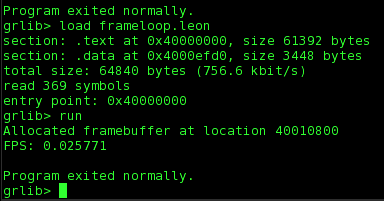
\includegraphics[scale=0.6]{../part4_files/Floating_Point_Grayscale_Screenshot.png}
	 		\caption{Floating Point Software Grayscale Conversion Results}
	 	\end{center}
	 \end{figure}
	 
	 \begin{figure}[H]
	 	\begin{center}
	 		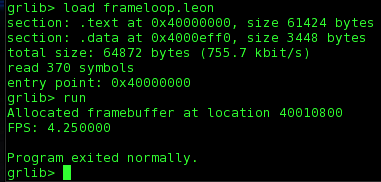
\includegraphics[scale=0.6]{../part4_files/Fixed_point_grayscale_resluts_screenshot.png}
	 		\caption{Fixed Point Software Grayscale Conversion Results}
	 	\end{center}
	 \end{figure}


%----------------------------------------------------------------------------------------
%	SECTION 3
%----------------------------------------------------------------------------------------
\section{Hardware Coprocessor - Grayscale Conversion}
In this section we were asked to read through the code in \textit{coproc.vhd} and \textit{coproc\_core.vhd} and provide a description of how the controller sends data to the core. After reading over the code in \textit{coproc.vhd} it became apparent that the LEON processor was passing the entire program instruction to the coprocessor. From there the coprocessor parses the instruction and extracts the op-code and source and destination register addresses. After getting the source register addresses it pulls the data directly from these registers. Therefore, the coprocessor has direct access to the LEON processor's registers. \\

We based our hardware coprocessor for the grayscale conversion on the logic we used to implement the software grayscale conversion. Here is a hardware diagram for the coprocessor we designed:

	 \begin{figure}[H]
	 	\begin{center}
	 		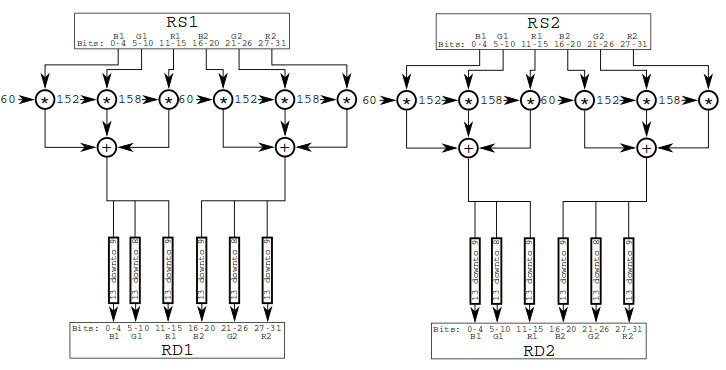
\includegraphics[scale=0.6]{../part5_files/Grayscale_coprocessor_dataflow.png}
	 		\caption{Hardware Grayscale Conversion Coprocessor Dataflow Diagram}
	 	\end{center}
	 \end{figure}

The structure for the hardware coprocessor ended up being fairly simple and easily parallelized. Because of these qualities we were able to make the coprocessor complete the operation in one clock cycle. Additionally, since we were able to output a 64-bit value from the coprocessor, we are able to process four individual pixels in that single clock cycle. Including the load and storing operations (for some reason we could only get the 32-bit load/store operations to work correctly) it would only take 5 clock cycles (assuming the load and store operations take one cycle each).

	 \begin{figure}[H]
	 	\begin{center}
	 		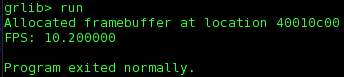
\includegraphics[scale=0.6]{../part5_files/Fixed_point_greyscale_coprocessor_results.png}
	 		\caption{Fixed Point Coprocessor Grayscale Conversion Results}
	 	\end{center}
	 \end{figure}




\subsection{Coprocessor Interface Instructions}
	The LDC - Load Coprocessor Register instruction loads a word (32-bits) from memory into a coprocessor register.\\
	
	The LDDC - Load Double Coprocessor Register instruction loads a double-word (64-bits) from memory into a coprocessor register pair.\\
	
	The STC - Store Coprocessor instruction stores the value of a coporcessor register into memory.\\
	
	The STDC - Store Double Coprocessor instruction stores the value of a coprocessory register pair (with consecutive odd and even addresses) into memory.\\
	
	The opcode for both the LD and ST class of operations is 11 but they are differentiated by their op3 value.\\
	
	The CPOP1 - Coprocessor Operate 8 bits (opcode + op3) to denote that the instruction needs to be executed on the coprocessor. The remaining 24 bits are used to signify the 2 source registers, 1 destination register and the operation to be performed. All the register addresses refer to the coprocessor registers.



%----------------------------------------------------------------------------------------
%	SECTION 4
%----------------------------------------------------------------------------------------
\section{Software Edge Detection}

For this part, we created a new Mode 5 to implement the edge detection in software. In this mode, we first called the software implementation of the grayscale conversion and then applied the Laplacian edge detector on the image, going left to right and top to bottom. We implemented this using two nested for loops, with the inner one traversing across the columns and the inner one traversing across the rows.\\

Here is a screenshot of our performance results of the software edge detection:

	 \begin{figure}[H]
	 	\begin{center}
	 		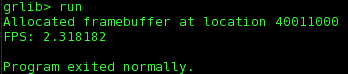
\includegraphics[scale=0.6]{../part6_files/Software_Laplace_edge_software_performance.png}
	 		\caption{Software Laplace Edge Detection Results}
	 	\end{center}
	 \end{figure}


%----------------------------------------------------------------------------------------
%	SECTION 5
%----------------------------------------------------------------------------------------
\section{Hardware Coprocessor - Edge Detection}
In this section, the task given is to modify the coprocessor to be able to perform greyscale edge detection. In order to implement this ability correctly, some changes had to be made to the files \textit{coproc.h}, \textit{coproc.vhd}, and \textit{coproc\_core.vhd}. The changes to the files were to provide two new instructions, CP\_PRELOAD, and CP\_EDGE\_DETECT.\\
In order to increase throughput, and potentially accelerate the process, the conclusion was made that the best approach to performing edge detection is as follows. Since the laplacian edge detection operation performed on a pixel requires the values of the eight pixels that surround it, a design decision made was that edge detection will not be performed on the pixels on the edge of the screen. Another design decision that was made was to load in six pixels at a time, to reduce the number of loads that were called, and allows for the loading and storing of 32-bit values. The six pixels that are loaded in to the coprocessor are the [$y - 1$][$x - 1$], [$y - 1$][$x$], [$y$][$x - 1$], [$y$][$x$], [$y + 1$][$x - 1$], and [$y + 1$][$x$] pixels used for the calculation. \\

Due to the pixel loading requirement outlined above, each time the algorithm reaches the next row in the frame, a set of six pixels have to be loaded at the beginning to guarantee correct edge detection. With this in mind, the instruction CP\_PRELOAD was created to perform just that, to load the first six pixels at the beginning of a new row. \\

Once the preload is complete, then the row is traversed to perform edge detection on each pixel in the row up to the second to last pixel. For each element in the row, grayscale conversion is performed on the six pixels, and the pixels are then loaded into the coprocessor through the CP\_EDGE\_DETECT instruction. The instruction performs the edge detection operation as shown in figure 6. \\

Another decision made was when the greyscale conversion of the pixels were performed, the greyscale pixels are stored in internal registers of the coprocessor as opposed to writing them out to a temporary framebuffer. This decision was made so that cycles would not be wasted reading and writing to external memory, also, there was no need to wait for the greyscale conversion to finish before edge detection was performed on the pixels. Using the hardware to perform the greyscale conversion, the instruction had to be called twice. Once with the top four pixels, then again with the bottom two pixels with random junk that is not used. Once conversion is complete, the registers that the greyscaled pixels are at are set as inputs to the CP\_EDGE\_DETECT instruction. Edge detection is performed on two adjacent pixels, and the result is returned as a 32-bit result.\\

	\begin{figure}[H]
		\begin{center}
			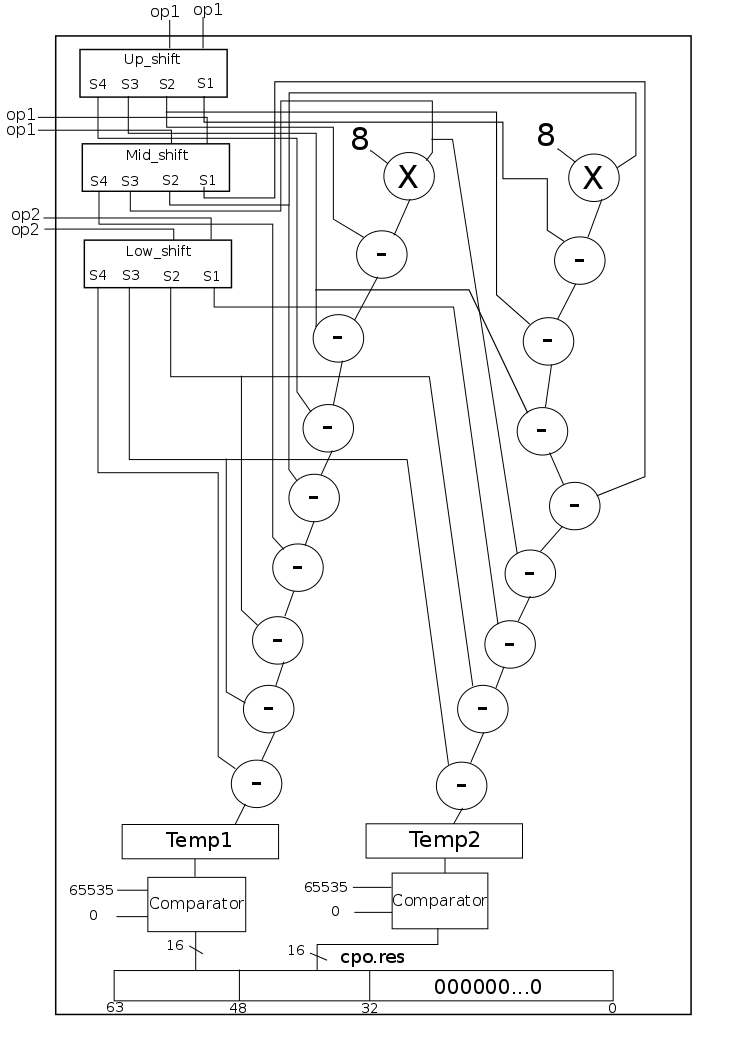
\includegraphics[scale=0.45]{./edge_detection.png}
			\caption{Hardware Laplace Edge Detection diagram}
		\end{center}
	\end{figure}

The decisions made that were outlined above have resulted in a speed up of 2.75 in the execution time of the operation, as shown in figure 7.

For the hardware edge detection implementation, we added two new opcodes - CP\_PRELOAD and 

CP\_EDGE\_DETECT. In coproc\_core, we essentially implemented 3 shift registers each being 64-bits long. Using CP\_PRELOAD, we shift in the next pixels to be apply the Laplacian edge detection on. 

CP\_EDGE\_DETECT consists of two cycles. In the first cycle, it performs the internal shifting of the shift registers and in the next cycle, it performs the Laplacian edge detection computation. Since we have 64-bit (4 pixels) shift registers, we are able to compute the Laplacian value for two center pixels simultaneously.\\

We perform our grayscale conversion in line with the edge detection computation, unlike the software implementation in which we first converted all the images to grayscale and then performed the edge detection. With the hardware implementation we were able to observe a 2.75 speedup when compared to the software implementation of the edge detection algorithm.\\

	 \begin{figure}[H]
	 	\begin{center}
	 		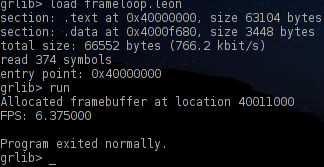
\includegraphics[scale=0.6]{../part7_files/Hardware_Laplace_edge_detection_performance.png}
	 		\caption{Hardware Laplace Edge Detection Results}
	 	\end{center}
	 \end{figure}



%----------------------------------------------------------------------------------------
%	SECTION 6
%----------------------------------------------------------------------------------------
\section{Conclusion}

Through this Machine Problem assignment, we learned about a general  hardware-software implementation and architecture.

%----------------------------------------------------------------------------------------
%	BIBLIOGRAPHY
%----------------------------------------------------------------------------------------
%\newpage

%\bibliographystyle{unsrt}

%\bibliography{sample}

%----------------------------------------------------------------------------------------


\end{document}
